\documentclass[border=1pt]{standalone}
\usepackage[usenames,dvipsnames]{xcolor}
\usepackage{tikz,array,comment}
\usepackage{tikz-qtree}
\usepackage{sansmath}
\usetikzlibrary{arrows,shapes,automata,patterns,trees,decorations}

\renewcommand{\familydefault}{\sfdefault}
\sffamily\sansmath

\begin{document}

% Set the overall layout of the tree
\tikzset{level 1/.style={level distance=10.0cm}}
\tikzset{level 2+/.style={level distance=1.6cm}}
\tikzset{edge from parent/.append style={->,line width=1.2,shorten >=2.5pt,shorten <=2.5pt}}
% Define styles for leafs
\tikzset{every leaf node/.style={draw,text width=1.09cm,inner sep=2pt,minimum height=0.4cm,align=center}}

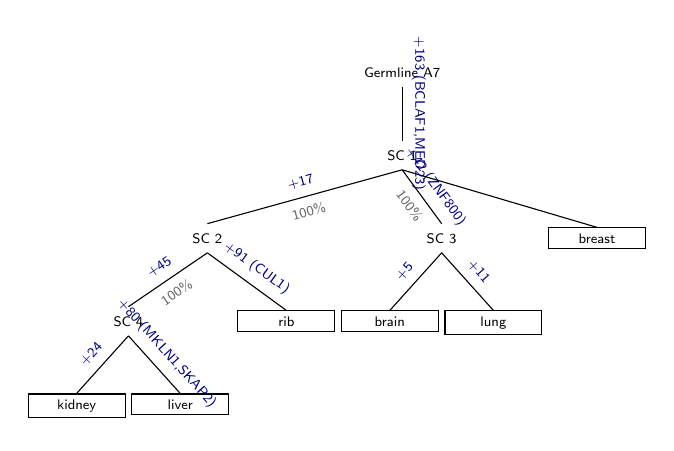
\begin{tikzpicture}[sloped,font=\sansmath\sffamily\normalsize]

\Tree [.\tiny{Germline~A7} 
	\edge node[above, NavyBlue]{\tiny{+163 (BCLAF1,MED23)}};
 	% Acquired mutations (163): -, -, -, -, -, -, -, -, -, -, -, -, -, -, -, -, -, -, -, -, -, -, -, -, -, -, -, -, -, -, -, AHCYL2, AK5, AMPH, AMPH, ARHGEF10L, ASAP3, AUTS2, AUTS2, AUTS2, AVL9, BAI2, BCLAF1, C1orf94, CACNA1A, CALCR, CALN1, CD53, CDC14A, CDCA7L, CHN2, CLDN1, CLSTN2, CLSTN2, CNTNAP2, COL24A1, COL28A1, COL28A1, CREB5, CROT, CYP2J2, CYP3A43, DGKI, DKFZp564N2472, DLG1, DLGAP3, ECOP, EIF3B, ENSG00000172400, ENSG00000172823, ENSG00000177133, ENSG00000184579, ENSG00000199627, ENSG00000204990, ENSG00000205695, ENSG00000210736, ENSG00000213650, ENSG00000216700, ENSG00000216737, ENSG00000216897, ENSG00000216897, ENSG00000218685, ENSG00000218772, ENSG00000220792, ENSG00000221777, ENSG00000222101, ENSG00000222435, ENSG00000222573, ENSG00000222929, EPB41L2, ERI3, EXOC4, EYA4, EZR, FAF1, FAM172A, FAM172A, FAM54A, FAM81B, FBXO30, FGGY, FKBP9L, FLJ36031, FZD1, GPSM2, GRIK3, GRIK3, GRM1, GRM1, GRM1, GRM1, GTF2H5, HDAC9, HMGB1L13, JHDM1D, KIF1B, LHX8, LOC100131512, LOC100131774, LOC100133118, LOC100134516, LOC100134662, LOC100134731, LOC126987, LOC393076, LOC645181, LOC645466, LOC645757, LOC653052, LOC728093, LOC729852, LRGUK, MAP3K13, MCF2L2, MED23, MEST, MRPS17, MYL10, NEGR1, NEGR1, NFIA, NXPH1, OMA1, PARK2, PPP1R9A, PTBP2, PTPRK, PTPRN2, PTPRN2, PUM1, RAPGEF5, RELN, RPL31P39, RSBN1, SCAMP1, SMARCD3, SND1, SNX9, SORT1, SRPK2, SUNC1, TSPAN33, TWISTNB
	% Acquired mutations (163): 19__13229344__X>Y, 1__100596975__X>Y, 1__10176897__X>Y, 1__102357816__X>Y, 1__104919770__X>Y, 1__105479711__X>Y, 1__105751148__X>Y, 1__105976500__X>Y, 1__106429293__X>Y, 1__109262628__X>Y, 1__109742485__X>Y, 1__111243855__X>Y, 1__114141754__X>Y, 1__17802653__X>Y, 1__23629267__X>Y, 1__25335187__X>Y, 1__2866642__X>Y, 1__31256719__X>Y, 1__31969094__X>Y, 1__34410048__X>Y, 1__35125075__X>Y, 1__37143587__X>Y, 1__37146830__X>Y, 1__4293949__X>Y, 1__44507311__X>Y, 1__47795503__X>Y, 1__50820201__X>Y, 1__5307845__X>Y, 1__55614612__X>Y, 1__58812365__X>Y, 1__59173150__X>Y, 1__59395273__X>Y, 1__59606236__X>Y, 1__60186271__X>Y, 1__61374740__X>Y, 1__66675643__X>Y, 1__72348627__X>Y, 1__72405199__X>Y, 1__75383214__X>Y, 1__77000685__X>Y, 1__77613234__X>Y, 1__82352086__X>Y, 1__86233044__X>Y, 1__88704682__X>Y, 1__95654758__X>Y, 1__97051849__X>Y, 1__98616638__X>Y, 3__141540851__X>Y, 3__141541946__X>Y, 3__179010668__X>Y, 3__183270834__X>Y, 3__184422096__X>Y, 3__186689735__X>Y, 3__190602791__X>Y, 3__191483297__X>Y, 3__198534921__X>Y, 5__100875880__X>Y, 5__100934674__X>Y, 5__77741526__X>Y, 5__84621724__X>Y, 5__84856901__X>Y, 5__88441860__X>Y, 5__88981104__X>Y, 5__91103592__X>Y, 5__91219445__X>Y, 5__91299931__X>Y, 5__91357738__X>Y, 5__91737547__X>Y, 5__91758970__X>Y, 5__92685911__X>Y, 5__93048746__X>Y, 5__93108774__X>Y, 5__94798178__X>Y, 5__98919500__X>Y, 6__128888781__X>Y, 6__131268132__X>Y, 6__131972080__X>Y, 6__132396420__X>Y, 6__133239118__X>Y, 6__133809460__X>Y, 6__134818453__X>Y, 6__134973299__X>Y, 6__136618559__X>Y, 6__136668368__X>Y, 6__140049282__X>Y, 6__140884297__X>Y, 6__146172510__X>Y, 6__146410871__X>Y, 6__146542099__X>Y, 6__146625698__X>Y, 6__146625699__X>Y, 6__158141272__X>Y, 6__158572652__X>Y, 6__159113832__X>Y, 6__162346313__X>Y, 6__165127699__X>Y, 7__101047598__X>Y, 7__103221094__X>Y, 7__104589345__X>Y, 7__10477769__X>Y, 7__106111173__X>Y, 7__109110120__X>Y, 7__11321150__X>Y, 7__124677955__X>Y, 7__127390523__X>Y, 7__128576668__X>Y, 7__128793132__X>Y, 7__129897913__X>Y, 7__130423905__X>Y, 7__131131116__X>Y, 7__132868898__X>Y, 7__133443482__X>Y, 7__135702941__X>Y, 7__136758689__X>Y, 7__139096025__X>Y, 7__139572873__X>Y, 7__140684659__X>Y, 7__140726554__X>Y, 7__144648965__X>Y, 7__146622310__X>Y, 7__150645364__X>Y, 7__155721074__X>Y, 7__157323232__X>Y, 7__157841987__X>Y, 7__17294379__X>Y, 7__18630770__X>Y, 7__19684407__X>Y, 7__20539353__X>Y, 7__20541601__X>Y, 7__21191092__X>Y, 7__21988837__X>Y, 7__22397215__X>Y, 7__2362179__X>Y, 7__25518368__X>Y, 7__25535588__X>Y, 7__26995271__X>Y, 7__28805042__X>Y, 7__29479373__X>Y, 7__32671620__X>Y, 7__38537806__X>Y, 7__38635352__X>Y, 7__47131612__X>Y, 7__48016189__X>Y, 7__51779387__X>Y, 7__53041859__X>Y, 7__55582402__X>Y, 7__55736464__X>Y, 7__55987397__X>Y, 7__56612832__X>Y, 7__69094162__X>Y, 7__69315563__X>Y, 7__69482807__X>Y, 7__70884677__X>Y, 7__7185556__X>Y, 7__7426061__X>Y, 7__7540276__X>Y, 7__7631972__X>Y, 7__8601313__X>Y, 7__86849072__X>Y, 7__90726410__X>Y, 7__93033408__X>Y, 7__94374627__X>Y, 7__99297850__X>Y
	% Acquired mutations (163): 1,2,10,14,17,20,22,23,27,28,33,36,37,39,43,44,47,61,62,64,65,67,68,70,74,76,78,79,81,84,90,108,109,110,111,113,115,119,123,124,125,126,130,132,137,138,139,142,144,145,146,148,149,150,151,158,159,160,163,164,170,171,177,178,180,181,189,190,193,194,196,199,201,204,205,208,209,211,212,213,214,219,220,224,226,227,228,229,231,233,234,236,237,238,239,244,245,247,248,249,253,256,257,261,268,271,272,273,274,275,276,277,279,283,287,293,298,306,307,311,314,316,318,323,327,330,331,332,333,334,337,344,351,355,356,359,363,364,372,374,375,386,387,390,402,407,411,413,415,418,419,423,428,431,434,441,442,445,446,448,453,464,465
	% VAF of acquired mutations: mean 33.07%; median 33.33%
	[.\tiny{SC~1} 
		\edge node[above, NavyBlue]{\tiny{+17}} node[below, black!60]{\tiny{100\%}};
 		% Acquired mutations (17): -, -, -, -, -, ENSG00000189015, ENSG00000200288, FAM174A, FLJ42291, LEPR, NTNG1, PGM1, POU6F2, PTPRS, ST6GALNAC3, UBE2U, ZNF716
		% Acquired mutations (17): 19__5285005__X>Y, 1__107451172__X>Y, 1__28295035__X>Y, 1__56623876__X>Y, 1__63860983__X>Y, 1__64441504__X>Y, 1__65668049__X>Y, 1__76627049__X>Y, 1__83148267__X>Y, 2__112081674__X>Y, 3__178790327__X>Y, 5__91448176__X>Y, 5__99983739__X>Y, 7__12163423__X>Y, 7__152796034__X>Y, 7__39028384__X>Y, 7__57562948__X>Y
		% Acquired mutations (17): 26,52,66,86,95,200,202,246,259,296,385,398,401,416,451,466,474
		% VAF of acquired mutations: mean 33.78%; median 35.68%
		[.\tiny{SC~2} 
			\edge node[above, NavyBlue]{\tiny{+45}} node[below, black!60]{\tiny{100\%}};
 			% Acquired mutations (45): -, -, -, -, -, -, ABCA13, AGBL4, ATG10, C1orf94, CDA, DOCK7, ENSG00000219806, ENSG00000222929, FAM172A, FGFR1OP, FHAD1, FOXP2, GNG7, GUCA2A, HIPK1, HIVEP2, ITGB1BP3, LOC100129148, LOC100130332, LOC100132224, LOC100132918, LOC100134778, LOC100134791, LOC391044, LOC729920, LPHN2, LPHN2, LRRIQ3, MYOM3, NAMPT, NRF1, OMA1, PRDM16, PRDM2, SLC44A5, SNX13, TCF21, THSD7A, ZSCAN20
			% Acquired mutations (45): 19__2659768__X>Y, 19__3892001__X>Y, 1__105379245__X>Y, 1__114219566__X>Y, 1__14012851__X>Y, 1__15514080__X>Y, 1__20764200__X>Y, 1__24281964__X>Y, 1__2984058__X>Y, 1__33685697__X>Y, 1__34418559__X>Y, 1__42406647__X>Y, 1__49633137__X>Y, 1__58771777__X>Y, 1__59281345__X>Y, 1__62947849__X>Y, 1__74240020__X>Y, 1__75465843__X>Y, 1__81746027__X>Y, 1__82206699__X>Y, 3__183672363__X>Y, 3__190153999__X>Y, 5__100982495__X>Y, 5__81305602__X>Y, 5__93269376__X>Y, 5__96862610__X>Y, 6__134204985__X>Y, 6__139970758__X>Y, 6__143071684__X>Y, 6__167353536__X>Y, 7__105706428__X>Y, 7__113907477__X>Y, 7__11500805__X>Y, 7__129004987__X>Y, 7__135254114__X>Y, 7__138787055__X>Y, 7__155526899__X>Y, 7__16156793__X>Y, 7__17798775__X>Y, 7__24059182__X>Y, 7__48231052__X>Y, 7__49282561__X>Y, 7__50292215__X>Y, 7__52781875__X>Y, 7__52977271__X>Y
			% Acquired mutations (45): 31,32,45,59,77,91,100,105,117,133,143,186,223,232,243,252,254,260,263,278,281,282,286,302,304,308,309,321,322,326,338,340,342,347,366,367,384,388,404,406,440,444,456,458,477
			% VAF of acquired mutations: mean 32.29%; median 28.07%
			[.\tiny{SC~4} 
				\edge node[above, NavyBlue]{\tiny{+24}};
 				% Acquired mutations (24): -, -, -, -, -, AADACL3, C6orf190, CNTNAP2, CNTNAP2, CNTNAP2, DAB1, ECE2, FAF1, FGF12, GPR31, KIAA1026, LAMB4, LHFPL3, LPHN2, LRRC7, NCAPG2, SAMD3, TARP, uc010lit.1
				% Acquired mutations (24): 1__12659643__X>Y, 1__15161769__X>Y, 1__50946188__X>Y, 1__58312966__X>Y, 1__70014881__X>Y, 1__81903009__X>Y, 3__179526416__X>Y, 3__185485452__X>Y, 3__193844821__X>Y, 6__128208030__X>Y, 6__130671400__X>Y, 6__167498834__X>Y, 7__102599349__X>Y, 7__103863521__X>Y, 7__107452067__X>Y, 7__131202501__X>Y, 7__144631667__X>Y, 7__145499555__X>Y, 7__146911774__X>Y, 7__147495911__X>Y, 7__158145739__X>Y, 7__38316335__X>Y, 7__49622553__X>Y, 7__66651915__X>Y
				% Acquired mutations (24): 5,16,57,58,73,96,135,152,153,154,172,188,241,251,265,291,295,297,343,345,370,432,455,470
				% VAF of acquired mutations: mean 20.96%; median 21.19%
				\node[black,draw,text width=1.09cm,inner sep=2pt,align=center]{\tiny{kidney}};  
				% Present mutations: 249; Reported mutations: 249 
				\edge node[above, NavyBlue]{\tiny{+80 (MKLN1,SKAP2)}};
 				% Acquired mutations (80): -, -, -, -, -, -, -, -, -, -, -, -, -, -, -, AASS, ABCA13, ABCA4, ARHGAP29, ASB4, AUTS2, BARHL2, CLCN6, COL16A1, COL24A1, CSMD2, CSMD2, DEFB131, DGKG, DGKI, DNAJB6, DPYD, ELMO1, ENSG00000172823, ENSG00000182965, ENSG00000200601, ENSG00000207247, ENSG00000216966, ENSG00000218896, ENSG00000220792, FAF1, FBXO30, GPR85, KIF25, LOC100128081, LOC100131199, LOC100133111, LOC100134549, LOC100134742, LOC554248, LPHN2, LRRC7, MAP3K5, MASP1, MEST, MKLN1, NASP, NCAPG2, NEGR1, NFIA, NHLH2, NPSR1, NPTX2, NPVF, PARK2, PARK2, PAX7, PCSK1, PDE7B, PEX5L, PIK3CG, PTPRK, PTPRN2, RPS6KA1, RPS6KA2, SASS6, SERAC1, SKAP2, TCTEX1D1, ZNF212
				% Acquired mutations (80): 1__100350285__X>Y, 1__105779592__X>Y, 1__106490664__X>Y, 1__116184351__X>Y, 1__11799962__X>Y, 1__18928257__X>Y, 1__25329446__X>Y, 1__26747401__X>Y, 1__30752765__X>Y, 1__31936651__X>Y, 1__34147858__X>Y, 1__34262945__X>Y, 1__4367117__X>Y, 1__45855628__X>Y, 1__50948218__X>Y, 1__61295653__X>Y, 1__67009131__X>Y, 1__69288072__X>Y, 1__69771032__X>Y, 1__71881803__X>Y, 1__73952156__X>Y, 1__81737245__X>Y, 1__86142745__X>Y, 1__90973618__X>Y, 1__94229729__X>Y, 1__94515716__X>Y, 1__98075740__X>Y, 2__112148096__X>Y, 3__181190420__X>Y, 3__187486758__X>Y, 3__188480934__X>Y, 3__196174967__X>Y, 4__9053068__X>Y, 5__51939810__X>Y, 5__88576328__X>Y, 5__95751619__X>Y, 5__96986124__X>Y, 6__128364136__X>Y, 6__133449351__X>Y, 6__136421335__X>Y, 6__137001899__X>Y, 6__137290849__X>Y, 6__143749402__X>Y, 6__146186567__X>Y, 6__148074549__X>Y, 6__158545732__X>Y, 6__162159061__X>Y, 6__162682987__X>Y, 6__165264097__X>Y, 6__166841984__X>Y, 6__167553070__X>Y, 6__168173437__X>Y, 7__106336549__X>Y, 7__111989127__X>Y, 7__112487100__X>Y, 7__121619930__X>Y, 7__129914387__X>Y, 7__130802135__X>Y, 7__137171774__X>Y, 7__140733376__X>Y, 7__148554467__X>Y, 7__156841870__X>Y, 7__157532394__X>Y, 7__158120776__X>Y, 7__15885801__X>Y, 7__166598__X>Y, 7__20956773__X>Y, 7__25240044__X>Y, 7__25400320__X>Y, 7__26663040__X>Y, 7__28201971__X>Y, 7__34693256__X>Y, 7__37249595__X>Y, 7__48361048__X>Y, 7__48407719__X>Y, 7__6665240__X>Y, 7__69204907__X>Y, 7__9420732__X>Y, 7__94920150__X>Y, 7__98132047__X>Y
				% Acquired mutations (80): 3,4,6,7,9,12,29,30,35,38,41,51,60,85,92,97,99,101,112,116,121,127,147,156,157,167,168,173,174,175,183,187,191,195,197,203,206,215,221,225,240,250,267,294,299,305,310,315,319,329,341,346,352,354,358,361,368,369,373,376,378,379,381,382,389,391,392,393,396,397,399,409,412,429,430,433,435,437,457,473
				% VAF of acquired mutations: mean 19.18%; median 17.29%
				\node[black,draw,text width=1.09cm,inner sep=2pt,align=center]{\tiny{liver}};  
				% Present mutations: 305; Reported mutations: 305 
			]
			\edge node[above, NavyBlue]{\tiny{+91 (CUL1)}};
 			% Acquired mutations (91): -, -, -, -, -, -, -, -, -, -, -, -, -, -, -, -, -, -, ABCA13, ABCB1, ADH5P2, AGK, ATXN7L1, AUTS2, AUTS2, BCAR3, C1orf174, C6orf103, CCDC129, CD53, CNTNAP2, COL9A2, CRYGS, CRYZ, CUL1, DGKI, DLD, DNAH11, DOCK4, DOCK4, ELTD1, ENSG00000209101, ENSG00000214807, ENSG00000218053, ENSG00000218199, ENSG00000222576, ETV1, FHAD1, FLJ36031, GPR126, GPR31, GRB10, GRB10, HS2ST1, IGSF21, KIAA1026, LOC100128444, LOC100133128, LOC100134750, LOC388630, LOC728666, LOC729070, MACF1, MAGEF1, MAN1C1, MOSPD3, MYOM3, NDUFA4, NFIA, NPSR1, NRD1, PDCD2, PLAGL1, PTGER3, PTPRK, RBM15, RELN, RELN, RNF11, SLC25A24, SNX10, SOSTDC1, ST6GALNAC3, SYT6, TMEM195, TMEM207, TNFSF9, UBXN7, ZBTB40, ZNF804B, uc003kkn.1
			% Acquired mutations (91): 19__6482745__X>Y, 1__105239364__X>Y, 1__105993905__X>Y, 1__108455372__X>Y, 1__110640188__X>Y, 1__111238905__X>Y, 1__111729230__X>Y, 1__114435427__X>Y, 1__14978938__X>Y, 1__15589662__X>Y, 1__18536630__X>Y, 1__22697642__X>Y, 1__24267368__X>Y, 1__25927527__X>Y, 1__30270899__X>Y, 1__34845686__X>Y, 1__3814510__X>Y, 1__39593016__X>Y, 1__40603735__X>Y, 1__48261724__X>Y, 1__51486990__X>Y, 1__52065812__X>Y, 1__5461427__X>Y, 1__55895291__X>Y, 1__61454579__X>Y, 1__66684006__X>Y, 1__71240949__X>Y, 1__75016452__X>Y, 1__76645903__X>Y, 1__79175800__X>Y, 1__79782783__X>Y, 1__87222665__X>Y, 1__93820691__X>Y, 3__185957865__X>Y, 3__187702250__X>Y, 3__191648442__X>Y, 3__197642331__X>Y, 4__8990687__X>Y, 5__52005691__X>Y, 5__88564993__X>Y, 5__93725443__X>Y, 6__126988664__X>Y, 6__128840172__X>Y, 6__131099587__X>Y, 6__132498090__X>Y, 6__140428469__X>Y, 6__140762083__X>Y, 6__142699775__X>Y, 6__144414900__X>Y, 6__146941806__X>Y, 6__148147186__X>Y, 6__167492553__X>Y, 6__169212522__X>Y, 6__170755923__X>Y, 7__100050644__X>Y, 7__103095628__X>Y, 7__103149549__X>Y, 7__103484511__X>Y, 7__105043200__X>Y, 7__106055114__X>Y, 7__107333266__X>Y, 7__10939342__X>Y, 7__111460900__X>Y, 7__111615971__X>Y, 7__112003332__X>Y, 7__136950737__X>Y, 7__13981990__X>Y, 7__140921165__X>Y, 7__145047692__X>Y, 7__145761123__X>Y, 7__147977700__X>Y, 7__149289180__X>Y, 7__15592530__X>Y, 7__15953918__X>Y, 7__16530977__X>Y, 7__17180429__X>Y, 7__21031229__X>Y, 7__21893479__X>Y, 7__26273927__X>Y, 7__31635730__X>Y, 7__34854167__X>Y, 7__36805174__X>Y, 7__48636162__X>Y, 7__50743611__X>Y, 7__50762938__X>Y, 7__69765464__X>Y, 7__69780337__X>Y, 7__87153287__X>Y, 7__88539094__X>Y, 7__92466088__X>Y, 7__96061728__X>Y
			% Acquired mutations (91): 13,15,24,40,42,46,48,49,55,63,69,72,75,80,82,83,88,89,98,102,103,107,118,120,122,128,131,134,140,141,155,161,165,166,169,176,179,182,184,185,192,207,210,216,217,230,235,255,258,264,266,269,270,284,285,290,301,312,320,325,335,336,348,349,350,362,365,371,377,380,383,394,400,408,410,421,422,424,426,439,443,447,450,454,459,460,461,467,468,472,476
			% VAF of acquired mutations: mean 34.47%; median 35.77%
			\node[black,draw,text width=1.09cm,inner sep=2pt,align=center]{\tiny{rib}};  
			% Present mutations: 271; Reported mutations: 271 
		]
		\edge node[above, NavyBlue]{\tiny{+42 (ZNF800)}} node[below, black!60]{\tiny{100\%}};
 		% Acquired mutations (42): -, -, -, -, -, -, -, -, -, -, -, -, -, ASAP3, BCAR3, CPA2, ENSG00000184579, FAM133B, GIMAP2, KCNAB2, KCND2, KIAA1244, LOC100134513, LOC149351, LOC401296, LOC730338, MAP7, MEF2C, MET, PPP1R9A, PRDM2, PTPRN2, PTPRZ1, RAPGEF5, REPS1, RNF146, SHPRH, STX7, TP63, WNT2, ZNF800, uc003vzn.2
		% Acquired mutations (42): 1__13969946__X>Y, 1__23657742__X>Y, 1__5200289__X>Y, 1__6078316__X>Y, 1__88012472__X>Y, 1__91070565__X>Y, 1__93854947__X>Y, 3__183939925__X>Y, 3__191029472__X>Y, 5__100487032__X>Y, 5__51897782__X>Y, 5__52646559__X>Y, 5__88152359__X>Y, 6__127585527__X>Y, 6__132877609__X>Y, 6__136865483__X>Y, 6__138631562__X>Y, 6__139334982__X>Y, 6__146310991__X>Y, 6__164009292__X>Y, 6__165086154__X>Y, 7__112057194__X>Y, 7__116191247__X>Y, 7__116723056__X>Y, 7__119939380__X>Y, 7__121389154__X>Y, 7__126817485__X>Y, 7__129709116__X>Y, 7__141970436__X>Y, 7__144553427__X>Y, 7__149996770__X>Y, 7__155536914__X>Y, 7__157777596__X>Y, 7__1743704__X>Y, 7__22404575__X>Y, 7__26990797__X>Y, 7__27709540__X>Y, 7__46287907__X>Y, 7__46668790__X>Y, 7__67421751__X>Y, 7__92037109__X>Y, 7__94747583__X>Y
		% Acquired mutations (42): 0,8,11,18,19,21,25,50,54,56,87,93,94,114,129,162,198,242,262,288,289,292,313,324,328,339,353,357,360,403,405,414,417,420,425,427,436,452,462,469,471,475
		% VAF of acquired mutations: mean 40.14%; median 37.43%
		[.\tiny{SC~3} 
			\edge node[above, NavyBlue]{\tiny{+5}};
 			% Acquired mutations (5): -, AGBL4, AGBL4, HDAC9, ST6GALNAC3
			% Acquired mutations (5): 1__49111131__X>Y, 1__49210849__X>Y, 1__72822982__X>Y, 1__76492623__X>Y, 7__18977783__X>Y
			% Acquired mutations (5): 71,104,106,280,449
			% VAF of acquired mutations: mean 22.40%; median 20.63%
			\node[black,draw,text width=1.09cm,inner sep=2pt,align=center]{\tiny{brain}};  
			% Present mutations: 210; Reported mutations: 216 
			\edge node[above, NavyBlue]{\tiny{+11}};
 			% Acquired mutations (11): -, -, C6orf191, ENSG00000218484, ENSG00000219178, LOC100128444, LOC100129289, LOC100134670, PDE1C, SLC13A1, TSPAN12
			% Acquired mutations (11): 1__29727073__X>Y, 1__80531792__X>Y, 6__130205896__X>Y, 7__118709984__X>Y, 7__120300316__X>Y, 7__122574089__X>Y, 7__144547471__X>Y, 7__32019297__X>Y, 7__8838677__X>Y, 7__89920941__X>Y, 7__96066687__X>Y
			% Acquired mutations (11): 34,53,136,218,222,300,303,317,395,438,463
			% VAF of acquired mutations: mean 29.04%; median 29.66%
			\node[black,draw,text width=1.09cm,inner sep=2pt,align=center]{\tiny{lung}};  
			% Present mutations: 216; Reported mutations: 245 
		]
		\edge node[above, NavyBlue]{};
		\node[black,draw,text width=1.09cm,inner sep=2pt,align=center]{\tiny{breast}};  
		% Present mutations: 163; Reported mutations: 163 
	]
]

\end{tikzpicture}
% \caption{Phylogenetic tree illustrating the evolutionary history of the cancer. The derivation of an evolutionarily-compatible maximum likelihood tree identified 0 putative false-positives or false-negatives (out of 2868; 0.0%). Putative false-positives 0, put. false-negatives 0, put. false neg.-unknowns 0. }
\end{document}
